\documentclass[11pt,a4paper]{article}
\usepackage{fontspec}
\setmainfont{TeX Gyre Pagella}
\setsansfont{TeX Gyre Heros}
\usepackage[ngerman]{babel}
\usepackage[babel]{csquotes}
\usepackage[a4paper,margin=2.6cm]{geometry}
\usepackage{microtype}
\usepackage{graphicx}
\usepackage{booktabs}
\usepackage{array}
\usepackage{unicode-math}
\setmathfont{texgyrepagella-math.otf}
\usepackage{siunitx}
\sisetup{output-decimal-marker={,}, group-separator={.}, table-number-alignment=center, input-symbols={()}, table-align-text-post=false, mode=text}
\usepackage[font=small,labelfont={bf,sf},textfont=sf,justification=raggedright,singlelinecheck=false,skip=4pt]{caption}
\captionsetup[figure]{name=Abbildung}
\usepackage{titlesec}
\titleformat{\section}{\normalfont\sffamily\bfseries\large}{}{0pt}{}
\titlespacing*{\section}{0pt}{1.4em}{0.5em}
\usepackage{enumitem}
\usepackage[hidelinks]{hyperref}
\usepackage{xurl}
\usepackage{setspace}
\setstretch{1.12}
\setlength{\emergencystretch}{1.5em}
\newenvironment{figurenotes}{\par\vspace{2pt}\footnotesize\raggedright}{\par}
\newenvironment{tablenotes}{\par\vspace{4pt}\footnotesize\raggedright}{\par}
\newenvironment{literatur}{\begin{list}{}{\setlength{\leftmargin}{1.5em}\setlength{\itemindent}{-1.5em}\setlength{\itemsep}{0.35em}\small}\raggedright}{\end{list}}
\hypersetup{pdftitle={Wann das Parlament über Preise spricht},pdfauthor={Wolf-Fabian Hungerland},pdflang={de-DE}}

\begin{document}
\begin{flushleft}
{\sffamily\bfseries\LARGE Wann das Parlament über Preise spricht\par}
\vspace{0.4em}
{\sffamily\large Eine Aufmerksamkeitsreihe für den Bundestag, 1949 bis 2025\par}
\vspace{1em}
{\sffamily Wolf-Fabian Hungerland\footnote{Der Beitrag gibt die persönliche Auffassung des Autors wieder. Daten und Skripte: \url{https://github.com/hungerland-macro/PREISREDE}.}\par}
\vspace{0.3em}
{\sffamily\small Fassung vom 25.~November 2026\par}
\end{flushleft}
\vspace{0.8em}
\noindent\begin{minipage}{\linewidth}\small
\textsf{\textbf{Abstract.}} Der Beitrag zählt Preis- und Inflationswörter in allen 4.610 Plenarprotokollen des Bundestages von 1949 bis 2025. Die Reihe folgt den großen Inflationsschüben; die Gipfel 1973 und 2022 sind fast gleich hoch. In ruhigen Jahren spricht das Parlament seit etwa 2000 nur noch rund 40~\% so oft über das Preisniveau wie in den 1950er und 1960er Jahren, bei ähnlich niedrigen Raten. Das gilt auch für reinen Redetext, gemessen an anderen Makrothemen und für alle großen Fraktionen. Aus einem Dauerthema der Bonner Republik wurde ein Thema für Schübe. Zugleich verschob sich die Debatte zu Energiepreisen, während Wörter der staatlichen Preis- und Lohnsteuerung fast verschwanden.\par\vspace{0.4em}
\textsf{\textbf{JEL:}} E31, E58, N14
\end{minipage}
\vspace{0.6em}



\section{Warum parlamentarische Aufmerksamkeit messen}

Inflation ist eine Größe der Statistik und zugleich ein Gegenstand politischen Streits. Ob und wann dieser Streit stattfindet, bestimmt mit, unter welchem Druck Geldpolitik, Tarifparteien und Regierung stehen. Die Forschung zur Inflationsaufmerksamkeit misst fast nur private Haushalte und Medien: Suchanfragen und Twitter (Korenok et al., 2026), Nennungen in Zeitungen (Lamla \& Lein, 2014; Aarab et al., 2025), Antwortmuster in Umfragen (Bracha \& Tang, 2025). Aufmerksamkeit ist dabei mehr als eine Messfrage, denn sie verändert die Wirkung der Geldpolitik (Pfäuti, 2025). Das Parlament ist weitgehend unbeachtet geblieben. Textanalysen gibt es zum Bundestag für Fiskalpolitik (Latifi et al., 2024) und Zukunft (Küsters \& Andritzky, 2024), zu Anhörungen von Zentralbanken (Fraccaroli et al., 2020) und zur Inflationsrhetorik kanadischer Abgeordneter (Rancourt et al., 2025); vergleichende Parlamentskorpora erschließen Rauh und Schwalbach (2020). Die deutsche Agenda-Forschung codiert Anfragen und Gesetze nach Politikfeldern, aber erst ab 1978 und nicht nach Inflation (Breunig \& Schnatterer, 2019).

Dieser Beitrag misst den Raum, den Preise und Inflation seit 1949 in den Reden des Bundestages einnehmen. Die Reihe ist erheblich länger als die vorliegenden Maße. Ihr Wert liegt weniger in der Reaktion auf einzelne Inflationsraten als im historischen Wandel der Grundaufmerksamkeit. Die Agenda-Forschung beschreibt Aufmerksamkeit als Folge von Schüben und Abklingen (Downs, 1972; Jones \& Baumgartner, 2005); die Reihe zeigt, dass sich auch das Niveau zwischen den Schüben verschieben kann.

\section{Daten und Maß}

Grundlage sind die Plenarprotokolle aus dem Corpus der Plenarprotokolle des Deutschen Bundestages (CPP-BT) von Sean Fobbe (2026), Fassung vom 19. September 2026, veröffentlicht unter CC0. Der Korpus umfasst 4.653 Protokolle der 1. bis 21. Wahlperiode. Die Schätzungen nutzen die vollen Jahre 1949 bis 2025 mit 4.610 Protokollen; die 43 Sitzungen von Januar bis September 2026 zeigt Abbildung~\ref{fig:1} gesondert. Für jedes Protokoll zähle ich die Wörter und die Treffer eines Wortfelds und bilde Jahreswerte je Million Wörter. Die Normierung ist nötig, denn der Umfang schwankt zwischen 1,6 Mio. Wörtern 1961 und 7,0 Mio. Wörtern 2011.

Das Wortfeld erfasst das Preisniveau als Gesamtgröße: Inflation und ihre Zusammensetzungen, Deflation, Preisauftrieb, Preisniveau, Preisstabilität, Geldentwertung, Geldwertstabilität, Kaufkraftverlust und Lebenshaltungskosten. Einzelne Preise, etwa für Energie, Mieten oder Lebensmittel, zählen nicht mit, weil sie in jedem Politikfeld vorkommen. Sie laufen als eigenes Wortfeld mit, ebenso Placebo-Felder für andere Makrothemen.

Zur Prüfung der Trefferqualität wurde eine Zufallsstichprobe von 180 Treffern, 20 je Jahrzehnt, bewertet. Die Erstbewertung nahm das Sprachmodell Claude vor. 89~\% der Treffer meinen das allgemeine Preisniveau oder die Inflation, vor 1990 87~\%, danach 91~\%. Der Rest betrifft meist sektorale Preisniveaus oder übertragene Bedeutungen wie „Inflation von Konzepten“. Die Bewertung von 50 Treffern, darunter allen schwierigen Fällen, wiederholten ChatGPT, Gemini, DeepSeek und Claude blind. Fleiss' Kappa beträgt 0,90 über alle fünf Codierungen, 0,88 ohne die blinde Claude-Codierung und 0,93 unter den drei anderen Modellen allein. In drei Fällen, in denen alle vier Modelle anders urteilten, gilt ihr Urteil. Die Vollständigkeit prüft eine zweite Stichprobe: Fünf Sprachmodelle (ChatGPT, Gemini, DeepSeek, Grok, Claude) bewerteten blind 27 neue Treffer und 27 Zufallsstellen mit allgemeinen Preiswörtern wie Preis, Teuerung oder teurer, die das Wortfeld nicht erfasst (Fleiss' Kappa 0,96). Von den Treffern meinen 24 das Preisniveau. Von den übrigen Stellen meint es eine, eine Teuerungszulage von 1953. Hochgerechnet auf 23.475 Treffer und 131.098 Stellen ohne Treffer erfasst das Wortfeld damit rund vier Fünftel aller Stellen zum Preisniveau; bei nur einer Fundstelle reicht die Spanne von etwa der Hälfte bis fast zu allen. Die übersehene Stelle liegt vor 1990; dass das Wortfeld nach 1999 mehr übersieht, lässt sich damit weder zeigen noch ausschließen. Die Protokolle enthalten auch Fragestunden und schriftlich beantwortete Fragen. Komposita, die das Preisniveau nur mittelbar meinen, vor allem Inflationsausgleichsprämie und Inflationsausgleichsgesetz ab 2022, habe ich eigens geprüft: Ohne sie sinkt der Wert für 2022 von 372 auf 350, am Befund ändert das nichts.

Die Inflationsrate ist die jahresdurchschnittliche Veränderung gegenüber dem Vorjahr. Bis 1991 nutze ich den Preisindex für die Lebenshaltung der Vier-Personen-Haushalte von Arbeitern und Angestellten mit mittlerem Einkommen im früheren Bundesgebiet, weil nur er bis 1950 zurückreicht (Statistisches Bundesamt, 2023). Ab 1992 folgt der Verbraucherpreisindex für Deutschland (Statistisches Bundesamt, 2026).

\section{Befund 1: Die Debatte folgt den großen Schüben}

Abbildung~\ref{fig:1} zeigt beide Reihen. Die Gipfel liegen fast gleichauf: 371 Preiswörter je Million Wörter 1973 und 372 im Jahr 2022. Über den ganzen Zeitraum beträgt die Korrelation mit der Inflationsrate 0,57. Sie beruht aber fast ganz auf den Schüben: Ohne die Jahre 1970 bis 1975 und 2022 bis 2023 sinkt sie auf 0,26. Jenseits der Schübe sagt die Rate über die Debatte wenig.

\begin{figure}[tb]
\caption{Preiswörter im Plenum und Inflationsrate, 1949 bis 2025}\label{fig:1}
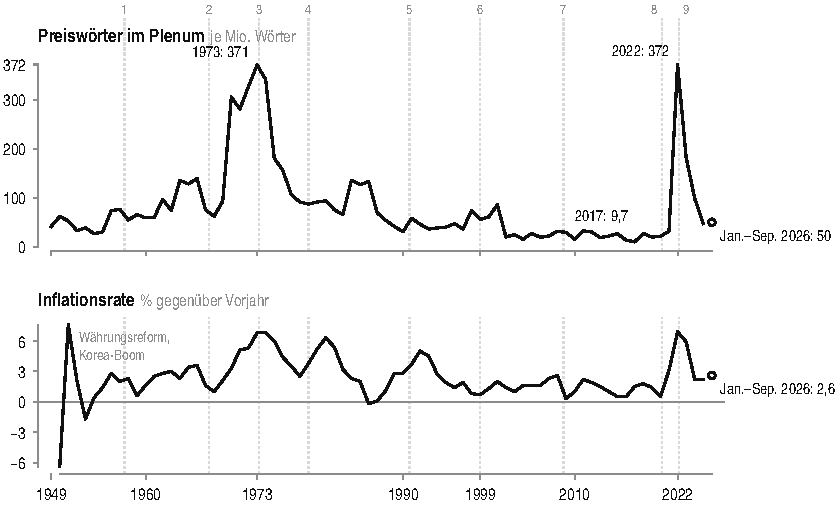
\includegraphics[width=\linewidth]{abbildungen/Abb1_Plenum_Inflation.pdf}
\begin{figurenotes}Oben: Treffer des Wortfelds Preisniveau je Million Wörter der Plenarprotokolle. Unten: Veränderung des Preisindex gegenüber dem Vorjahr, Jahresdurchschnitt. Hohle Punkte: Januar bis September 2026. Gestrichelt: 1 Bundesbankgesetz, 2 Stabilitätsgesetz, 3 Bretton Woods endet, erster Ölpreisschock, 4 zweiter Ölpreisschock, 5 Wiedervereinigung, 6 Euro, 7 Finanzkrise, 8 Corona, 9 Krieg gegen die Ukraine.\par\textit{Quellen:} Fobbe (2026); Statistisches Bundesamt; Deutsche Bundesbank; eigene Berechnungen.\end{figurenotes}
\end{figure}

Auffällig ist 1970: Die Reihe springt von 93 auf 306, während die Rate von 2,1~\% auf 3,3~\% stieg. Ob die Debatte der Rate vorauslief, zeigen Jahresdaten nicht. Sichtbar ist ihr Vorlauf im Vokabular: 1969 erreichten Wörter wie Aufwertung und Wechselkurs mit 259 je Million Wörter ihren Höchststand, nach 17 im Jahr 1967. Die Preisdebatte um 1970 begann als Debatte über importierte Inflation unter festen Wechselkursen, nicht über Energie.

\section{Befund 2: Das Grundniveau hat sich mehr als halbiert}

Der einfachste Vergleich braucht kein Modell. In Jahren mit Raten unter 3~\% kamen von 1953 bis 1969 im Median 64 Preiswörter auf eine Million Wörter, von 1999 bis 2025 noch 26, bei einer mittleren Rate dieser Jahre von 1,6~\% und 1,4~\%. Die Jahre 1953 bis 1969 folgen auf keinen großen Schub; das hohe frühe Niveau ist also kein bloßes Abklingen früherer Inflation. Auch die Verbreitung sank: Von den Reden mit mindestens 300 Wörtern enthielten in ruhigen Jahren vor 1999 im Median 4,5~\% ein Preiswort, von 1999 bis 2020 noch 1,8~\%. In den 1990er Jahren lag das Niveau mit 39 schon zwischen beiden Werten.

Tabelle~\ref{tab:1} schätzt die Reihe als Anpassungsmodell in Niveaus mit dem Vorjahreswert. Ein Strukturbruch darf das Niveau und die Reaktion auf die Rate verschieben. Ein Bruchtest über die Jahre 1975 bis 2005 wählt 2002 (p = 0,001, Bootstrap); die Konfidenzmenge nach dem Likelihood-Quotienten (Eo \& Morley, 2015) umfasst die Jahre 1999 bis 2004, nicht aber 1990. Spalte 1 nutzt 1999, das Jahr des Euro-Starts; Spalte 2 zeigt zum Vergleich 1990. Die Residuen sind nicht autokorreliert (Breusch-Godfrey, p > 0,17).

\begin{table}[tb]
\caption{Aufmerksamkeit und Inflationsrate, mit Strukturbruch}\label{tab:1}
\small
\begin{tabular*}{\linewidth}{@{\extracolsep{\fill}}>{\raggedright\arraybackslash}p{4.3cm}cccc@{}}
\toprule
Erklärende Größe & {\footnotesize\shortstack{(1)\\ Bruch 1999}} & {\footnotesize\shortstack{(2)\\ Bruch 1990}} & {\footnotesize\shortstack{(3)\\ nur Redetext}} & {\footnotesize\shortstack{(4)\\ ohne 1951/52 und 2021/23}} \\
\midrule
Inflationsrate & 0,060 & 0,078 & 0,062 & 0,062 \\
 & {\footnotesize(0,079)} & {\footnotesize(0,037)} & {\footnotesize(0,083)} & {\footnotesize(0,052)} \\
Rate, zusätzlich ab Bruch & 0,240 & 0,142 & 0,255 & 0,125 \\
 & {\footnotesize(0,000)} & {\footnotesize(0,110)} & {\footnotesize(0,000)} & {\footnotesize(0,119)} \\
Niveau, zusätzlich ab Bruch & $-$0,769 & $-$0,655 & $-$0,757 & $-$0,567 \\
 & {\footnotesize(0,000)} & {\footnotesize(0,009)} & {\footnotesize(0,000)} & {\footnotesize(0,000)} \\
Vorjahreswert, log & 0,588 & 0,550 & 0,582 & 0,645 \\
 & {\footnotesize(0,000)} & {\footnotesize(0,000)} & {\footnotesize(0,000)} & {\footnotesize(0,000)} \\
Langfristwert bei 2~\% & 70 / 34 & 76 / 33 & 82 / 45 & 73 / 30 \\
\midrule
Beobachtungen & 75 & 75 & 75 & 70 \\
$R^2$ & 0,75 & 0,73 & 0,73 & 0,78 \\
\bottomrule
\end{tabular*}
\begin{tablenotes}Abhängige Größe ist der Logarithmus der Treffer je Million Wörter, Jahre 1951 bis 2025. Konstante nicht ausgewiesen. In Klammern p-Werte, HAC-Standardfehler mit drei Lags. Langfristwert: Treffer je Million Wörter im Gleichgewicht bei einer Rate von 2~\%, vor und ab dem Bruch. Spalte 3: nur Redetext, bis 2021 aus Open Discourse (Richter et al., 2023), ab 2022 aus dem Reden-Datensatz des CPP-BT; in den gemeinsamen Jahren 2014 bis 2021 liefern beide fast gleiche Werte. Spalte 4: Bruch 1999, ohne die Korea-Jahre und den jüngsten Schub.\par\textit{Quellen:} Fobbe (2026); Richter et al. (2023); Statistisches Bundesamt; eigene Berechnungen.\end{tablenotes}
\end{table}

Das Niveau ab dem Bruch ist in allen Spalten deutlich tiefer. Wie stark, hängt von der Rate ab, weil sich mit dem Niveau auch die Steigung verschiebt. Nach Spalte 1 liegt der Langfristwert nach dem Bruch bei 1~\% Inflation bei 28~\% des früheren Werts (90-\%-Band 17~\% bis 38~\%), bei 2~\% bei 49~\% (36~\% bis 73~\%); ab 3~\% lassen sich die Regime nicht mehr unterscheiden. Der Befund gilt also für ruhige Jahre, und dort trägt ihn auch der modellfreie Vergleich. Er bleibt, wenn man je eine der fünf Inflationsepisoden weglässt, den Index aller privaten Haushalte ab 1964 nutzt, die Höchstrate der vorangegangenen zehn Jahre als Maß des Inflationsgedächtnisses aufnimmt oder die Jahre 1990 bis 1998 mit der Maastricht-Debatte weglässt. Auch ohne die Wörter Preisstabilität und Geldwertstabilität ändert sich nichts.

Die stärkere Reaktion auf die Rate nach dem Bruch ist dagegen nicht gesichert. Ohne den jüngsten Schub halbiert sie sich und ist nicht mehr signifikant (Spalte 4); sie beruht auf einer Episode. Abbildung~\ref{fig:2} zeigt beides: Die Punktwolke nach 1999 liegt tiefer, ihre Steilheit tragen 2022 und 2023. Auch eine Schwelle, ab der die Debatte anspringt, wie sie Korenok et al. (2026) und Pfäuti (2024) für Haushalte bei 2~\% bis 4~\% finden, lässt sich nicht sichern: Eine Gittersuche ab 1990 findet 3,7~\%, liegt damit aber auf der Mindestbesetzung von fünf Jahren, und der Bootstrap nach Hansen (1996) verwirft das lineare Modell nicht (p = 0,14).

\begin{figure}[tb]
\caption{Preiswörter und Inflationsrate vor und ab 1999}\label{fig:2}
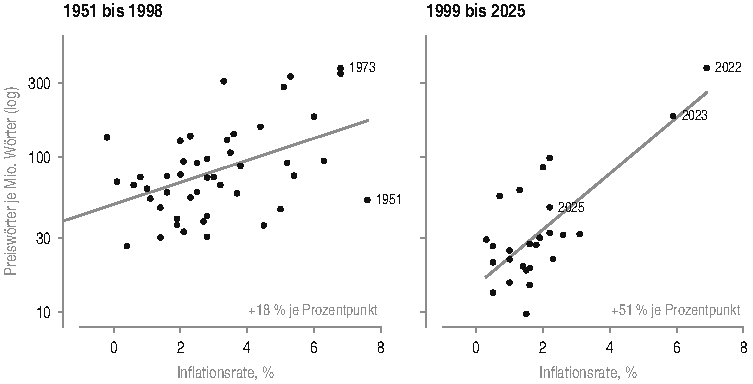
\includegraphics[width=\linewidth]{abbildungen/Abb2_Reaktion.pdf}
\begin{figurenotes}Jeder Punkt ist ein Jahr. Linie: Ausgleichsgerade des Logarithmus auf die Rate je Zeitraum.\par\textit{Quellen:} Fobbe (2026); Statistisches Bundesamt; eigene Berechnungen.\end{figurenotes}
\end{figure}

\section{Was die Halbierung nicht erklärt}

Drei mechanische Erklärungen liegen nahe; keine trägt. Erstens der Nenner: Die Protokolle enthalten Anlagen und Verfahrenstext, deren Anteil sich ändert. Auf reinem Redetext ist der Befund derselbe (Spalte 3). Zweitens eine breitere Tagesordnung, die jedes Thema verdünnt: In Jahren mit Raten unter 3~\% fielen im Redetext Wörter zu Arbeitslosigkeit, Haushalt und Wachstum nach 1999 nur auf 86~\% bis 98~\% ihres früheren Medians, Preiswörter auf 49~\%. Misst man die Preisrede an diesen drei Feldern, bleibt der Niveaubruch gesichert, auch ohne die Schübe (p = 0,04). Drittens ein anderes Vokabular für dasselbe: Ausdrücke wie Preissteigerung oder Teuerung gingen noch stärker zurück, von 35 auf 10 je Million Wörter.

Verschoben hat sich die Debatte dennoch. Wörter zu Energiepreisen, Preisbremsen und Heizkosten stiegen vom Median 6 je Million Wörter in den Jahren 1951 bis 1969 auf 59 in den Jahren 2010 bis 2021; 2022 erreichten sie 628. Seit 1999 spricht das Plenum über Preise vor allem als Energiepreise, über das Preisniveau nur im Schub. Wörter der staatlichen Preis- und Lohnsteuerung, etwa Konzertierte Aktion, Stabilitätsgesetz, Preisstopp und Lohnleitlinien, fielen in ruhigen Jahren auf ein Siebtel.

Wer spricht, zeigt eine Auswertung nach Fraktionen mit Open Discourse. In den Schüben redet die Opposition deutlich mehr über Preise als Regierung und Koalition, 1973 mit 905 gegen 263 Preiswörter je Million Wörter, 2022 mit 658 gegen 356. Hält man Partei und Jahr fest, sprechen Regierungsparteien rund 14~\% weniger über Preise als dieselben Parteien in der Opposition (p < 0,01); nach 1999 ändert sich dieser Abstand nicht. Der Rückgang des Grundniveaus trifft alle großen Fraktionen. In ruhigen Jahren sank der Median der CDU/CSU von 82 auf 36, der SPD von 73 auf 26 und der FDP von 74 auf 43. Neue Fraktionen mit anderen Themen erklären ihn nicht.

\section{Drei Lesarten}

Eine Lesart verbindet den Bruch mit der geldpolitischen Delegation: Mit der Währungsunion verschwand das Preisniveau aus dem Alltagsbetrieb und kehrt nur im Schub zurück. Dazu passt, dass die Konfidenzmenge des Bruchjahrs 1999 bis 2004 umfasst und nicht 1990. Die Aufmerksamkeit wanderte dabei teils zum Instrument: Wörter zu Zins und Geldpolitik stiegen nach 1999 in ruhigen Jahren um ein Viertel bis die Hälfte, und Politiker kommentieren die Geldpolitik der EZB meist mit dem Wunsch nach niedrigeren Zinsen (Ehrmann \& Fratzscher, 2011). Gegen die Lesart spricht, dass schon die Bank deutscher Länder ab 1948 und die Bundesbank ab 1957 von der Bundesregierung unabhängig waren.

Die zweite Lesart betont die Instrumente. Bis in die 1980er Jahre lag Preispolitik auch bei Parlament und Regierung, über das Stabilitätsgesetz von 1967, die Konzertierte Aktion und administrierte Preise. Preisstabilität war Teil des Parteienstreits, wie die Debatte über das deutsche Inflationstrauma zeigt (Barkhausen \& Teupe, 2025). Der Einbruch dieses Vokabulars stützt die Lesart; ihr Zeitpunkt passt aber schlechter, denn die Konzertierte Aktion endete schon 1977.

Die dritte Lesart ist international: Mit der Großen Moderation sanken Rate und Schwankung der Inflation fast überall, und die Erwartungen wurden fester verankert. Dann wäre der Rückgang kein deutscher oder europäischer Befund. Ein Land allein kann die drei Lesarten nicht trennen; dafür braucht es Parlamente außerhalb des Euroraums.

\section{Nach dem Schub von 2022}

Korenok und Munro (2024) finden, dass die Aufmerksamkeit von Haushalten nach dem Rückgang der Inflation zwei- bis dreimal so hoch bleibt wie vor dem Anstieg; die EZB beschreibt Ähnliches für Nachrichten (Aarab et al., 2025). Für den Bundestag ist ein solcher Überhang nicht zu sehen. 2025 lag die Reihe mit 47 Preiswörtern je Million Wörter zwar beim 2,4-Fachen des Mittels der Jahre 2015 bis 2020, die Rate aber mit 2,2~\% auch doppelt so hoch. Das Modell aus Spalte 1 erwartet für 2025 sogar 68, für Januar bis September 2026 genau den beobachteten Wert von 50. Das Parlament kehrte so schnell zum Grundniveau zurück, wie es die Rate erwarten lässt.

Ein methodischer Nebenbefund betrifft die parlamentarischen Anfragen. Unter allen 43.866 Kleinen und Großen Anfragen im Dokumentations- und Informationssystem für Parlamentsmaterialien (DIP) tragen nur 15 das Preisniveau oder seine Messung im Titel, von 1949 bis 1995 nur zwei, 1971 und 1972. Wer Inflationsaufmerksamkeit über Anfragetitel messen wollte, sähe den ersten Ölpreisschock nicht; die Inhalte von Anfragen codieren dagegen Kristensen et al. (2023).

\section{Was folgt daraus}

Erstens ein methodischer Punkt. Plenarprotokolle sind als Quelle für Aufmerksamkeitsmaße unterschätzt. Sie liegen maschinenlesbar und lückenlos seit 1949 vor, sind frei von Erhebungseffekten und messen, was politisch verhandelt wird, nicht was Haushalte wahrnehmen.

Zweitens ein wirtschaftshistorischer. Das Preisniveau war in der Bonner Republik ein Dauerthema des Parlaments und ist es seit etwa 2000 nicht mehr. Der Wandel betrifft alle Fraktionen und fällt zeitlich mit der Währungsunion zusammen; ob die Delegation, der Rückzug staatlicher Preissteuerung oder die weltweite Disinflation ihn trägt, bleibt offen. Ob die Aufmerksamkeit seither stärker auf Schübe reagiert, lässt sich mit einer einzigen Episode nicht sichern.

Drittens eine Hypothese zur Kontrolle der Geldpolitik. Wenn das Parlament bei Raten nahe dem Ziel kaum über das Preisniveau spricht, schützt das die Notenbank vor kurzfristigem Druck, lässt Abweichungen vom Ziel aber lange ohne Debatte über das Preisniveau. In den 2010er Jahren mit zu niedriger Inflation sprach der Bundestag eher über Zinsen als über Preise. Ob diese Stille Glaubwürdigkeit oder Desinteresse ausdrückt, zeigen die Daten nicht; der formale Ort der Rechenschaft der EZB ist ohnehin das Europäische Parlament.

\section{Grenzen}

Das Maß zählt Wörter, nicht Positionen. Es unterscheidet nicht, ob jemand vor Inflation warnt oder sie für überschätzt hält. Die Wortfelder sind eine Setzung. Trefferqualität und Vollständigkeit haben Sprachmodelle geprüft; eine menschliche Codierung steht aus, und die Schätzung der Vollständigkeit beruht auf einer kleinen Stichprobe. Die Schübe von 1973 und 2022 kamen auch über die Energiepreise; die Reihe trennt Aufmerksamkeit für das Preisniveau nicht vollständig von Aufmerksamkeit für Energie. Die Protokolle der frühen Wahlperioden stammen aus der Texterkennung; Lesefehler senken eher die frühen Werte und wirken damit gegen den Befund. Jahresdaten mit 75 Beobachtungen und wenigen Episoden erlauben keine Aussage über eine allgemeine Reaktionsfunktion. Ein Vergleich mit Parlamenten innerhalb und außerhalb des Euroraums würde zeigen, ob der Wandel deutsch, europäisch oder allgemein ist. Daten und Skripte liegen offen unter \url{https://github.com/hungerland-macro/PREISREDE}.

\section*{Hinweis zum Einsatz von KI}

Bei der Erstellung des Beitrags kam das Sprachmodell Claude (Anthropic) zum Einsatz. Es schrieb nach Vorgaben des Autors die Python-Skripte für den Abruf der Anfragen, die Wortzählungen, die Schätzungen und die Abbildungen, entwarf Teile des Textes, prüfte Zahlen und Literaturangaben gegen die Originalquellen und redigierte den Text. Es nahm die Erstbewertung der Trefferstichprobe vor und schlug die Einteilung der 78 Anfragen vor, die der Autor übernahm. Die blinde Wiederholung beider Bewertungen übernahmen ChatGPT, Gemini, DeepSeek und Claude in getrennten Sitzungen ohne Kenntnis der Erstcodierung; die Prüfung der Vollständigkeit zusätzlich Grok. Die Einteilung der Anfragen prüften vier Läufe derselben Modelle blind (Fleiss' Kappa 0,91). Fragestellung, Wortfelder, Deutung der Ergebnisse und die Endfassung verantwortet der Autor. Skripte und Daten liegen offen, sodass alle Ergebnisse nachgerechnet werden können.

\section*{Literatur}

\begin{literatur}
\item Aarab, I., Bańbura, M., Bobeica, E. \& Leguay, E. (2025). Monitoring attention to inflation in the news. \emph{Economic Bulletin}, 6/2025, Box 5. Europäische Zentralbank.

\item Barkhausen, D. \& Teupe, S. (2025). The German inflation trauma: Weimar's policy lessons between persistence and reconstruction. \emph{Jahrbücher für Nationalökonomie und Statistik}, \emph{245}(3), 269--332. \url{https://doi.org/10.1515/jbnst-2023-0045}

\item Bracha, A. \& Tang, J. (2025). Inflation levels and (in)attention. \emph{Review of Economic Studies}, \emph{92}(3), 1564--1594. \url{https://doi.org/10.1093/restud/rdae063}

\item Breunig, C. \& Schnatterer, T. (2019). Political agendas in Germany. In F. R. Baumgartner, C. Breunig \& E. Grossman (Hrsg.), \emph{Comparative policy agendas: Theory, tools, data} (S. 97--104). Oxford University Press. \url{https://doi.org/10.1093/oso/9780198835332.003.0010}

\item Downs, A. (1972). Up and down with ecology: The “issue-attention cycle”. \emph{The Public Interest}, \emph{28}, 38--50.

\item Ehrmann, M. \& Fratzscher, M. (2011). Politics and monetary policy. \emph{Review of Economics and Statistics}, \emph{93}(3), 941--960. \url{https://doi.org/10.1162/REST\_a\_00113}

\item Eo, Y. \& Morley, J. (2015). Likelihood-ratio-based confidence sets for the timing of structural breaks. \emph{Quantitative Economics}, \emph{6}(2), 463--497. \url{https://doi.org/10.3982/QE186}

\item Fobbe, S. (2026). \emph{Corpus der Plenarprotokolle des Deutschen Bundestages (CPP-BT)} (Version 2026-09-19) {[}Datensatz{]}. Zenodo. \url{https://doi.org/10.5281/zenodo.22844952}

\item Fraccaroli, N., Giovannini, A. \& Jamet, J.-F. (2020). \emph{Central banks in parliaments: A text analysis of the parliamentary hearings of the Bank of England, the European Central Bank and the Federal Reserve} (ECB Working Paper Nr. 2442). Europäische Zentralbank.

\item Hansen, B. E. (1996). Inference when a nuisance parameter is not identified under the null hypothesis. \emph{Econometrica}, \emph{64}(2), 413--430. \url{https://doi.org/10.2307/2171789}

\item Jones, B. D. \& Baumgartner, F. R. (2005). \emph{The politics of attention: How government prioritizes problems}. University of Chicago Press.

\item Korenok, O. \& Munro, D. (2024). \emph{The rockets and feathers of inflation attention} (GLO Discussion Paper Nr. 1463). Global Labor Organization.

\item Korenok, O., Munro, D. \& Chen, J. (2026). Inflation and attention thresholds. \emph{Review of Economics and Statistics}, \emph{108}(3), 842--850. \url{https://doi.org/10.1162/rest\_a\_01402}

\item Kristensen, T. A., Mortensen, P. B., Green-Pedersen, C. \& Seeberg, H. B. (2023). The policy agenda effects of problem indicators: A comparative study in seven countries. \emph{Journal of Public Policy}, \emph{43}(2), 240--260. \url{https://doi.org/10.1017/S0143814X22000307}

\item Küsters, A. \& Andritzky, J. (2024). Welche Rolle spielt das Thema Zukunft im Bundestag? \emph{Wirtschaftsdienst}, \emph{104}(4), 252--257. \url{https://doi.org/10.2478/wd-2024-0069}

\item Lamla, M. J. \& Lein, S. M. (2014). The role of media for consumers' inflation expectation formation. \emph{Journal of Economic Behavior \& Organization}, \emph{106}, 62--77. \url{https://doi.org/10.1016/j.jebo.2014.05.004}

\item Latifi, A., Naboka-Krell, V., Tillmann, P. \& Winker, P. (2024). Fiscal policy in the Bundestag: Textual analysis and macroeconomic effects. \emph{European Economic Review}, \emph{168}, 104827. \url{https://doi.org/10.1016/j.euroecorev.2024.104827}

\item Pfäuti, O. (2024). \emph{The inflation attention threshold and inflation surges} (arXiv:2308.09480). arXiv. \url{https://doi.org/10.48550/arXiv.2308.09480}

\item Pfäuti, O. (2025). Inflation -- who cares? Monetary policy in times of low attention. \emph{Journal of Money, Credit and Banking}, \emph{57}(5), 1211--1239. \url{https://doi.org/10.1111/jmcb.13145}

\item Rancourt, M.-A., Déry, A., Fortier-Chouinard, A. \& Dufresne, Y. (2025). Understanding politicians' discourse on inflation and cost of living in Canada. \emph{Parliamentary Affairs}. \url{https://doi.org/10.1093/pa/gsaf052}

\item Rauh, C. \& Schwalbach, J. (2020). \emph{The ParlSpeech V2 data set: Full-text corpora of 6.3 million parliamentary speeches in the key legislative chambers of nine representative democracies} {[}Datensatz{]}. Harvard Dataverse. \url{https://doi.org/10.7910/DVN/L4OAKN}

\item Richter, F., Koch, P., Franke, O., Kraus, J., Kuruc, F., Thiem, A., Högerl, J., Heine, S. \& Schöps, K. (2023). \emph{Open Discourse} (Version 4) {[}Datensatz{]}. Harvard Dataverse. \url{https://doi.org/10.7910/DVN/FIKIBO}

\item Statistisches Bundesamt. (2023). \emph{Verbraucherpreisindizes für Deutschland. Lange Reihen ab 1948} (Ausgabe Dezember 2022).

\item Statistisches Bundesamt. (2026). \emph{Verbraucherpreisindex für Deutschland, 2020 = 100, Jahresdurchschnitte} {[}Datensatz, abgerufen über die Zeitreihendatenbank der Deutschen Bundesbank, BBDP1.A.DE.N.VPI.C.A00000.I20.A{]}.
\end{literatur}

\end{document}
